\documentclass[a4paper,hidelinks,14pt]{extarticle}

\usepackage[utf8]{inputenc}
\usepackage[T2A]{fontenc}
\usepackage[english, russian]{babel}
\usepackage{lipsum}
\usepackage{amsmath}
\usepackage{amssymb}
\usepackage{amsfonts}
\usepackage{mathtools}
\usepackage{datetime}
\usepackage[pdftex]{graphicx}
\usepackage{indentfirst}
\usepackage{asymptote}
\usepackage{systeme}
\usepackage[dvipsnames]{xcolor}
\usepackage{lastpage}
\usepackage{fancybox,fancyhdr}
\usepackage{hyperref}
\usepackage[font={small,it}]{caption}
\fancyhead[L]{Лабораторная работа №5}
\fancyhead[C]{}
\fancyhead[R]{\textit{Фильтр Калмана}}
\fancyfoot[L]{}
\fancyfoot[C]{\thepage\space}
\fancyfoot[R]{}
\pagestyle{fancy}
\newcommand{\gt}{\textgreater}
\newcommand{\lt}{\textless}
\usepackage{listings}
\usepackage{xcolor}
\lstset{
    basicstyle=\ttfamily\small,
    keywordstyle=\color{blue},
    commentstyle=\color{gray},
    stringstyle=\color{red},
    numbers=left,
    numberstyle=\color[gray]{0.7}\ttfamily\small,
    stepnumber=1,
    numbersep=8pt,
    frame=single,
    showstringspaces=false,
    tabsize=4,
    breaklines=true
}
\usepackage{subcaption}

\begin{document}
	\begin{titlepage}
		\setlength{\parindent}{0ex}
		
		\begin{center}
			\textsc{
				\vspace{1ex}
                Научно-исследовательский университет ИТМО \\
				\vspace{0.5ex}
				Факультет систем управления и робототехники \\
				\vspace{0.5ex}
			}
		\end{center}
		
		\vspace{45mm}
		
		\begin{center}
			Отчет по лабораторной работе №5\\
			\textbf{Синтез оптимального наблюдателя \\
			Фильтр Калмана и ЛКГ-синтез} \\
			Вариант 21
		\end{center}
		
		\vspace{50mm}
		
		\begin{minipage}{.45\linewidth}
			Выполнил студент
            \\
			Проверил преподаватель
		\end{minipage}
		\hfill
		\begin{minipage}{.52\linewidth}
			\begin{flushright}
				Мовчан Игорь Евгеньевич, R3480
                \\
				Парамонов Алексей Владимирович
			\end{flushright}
		\end{minipage}
		
		\vfill
		\begin{center}
			Санкт-Петербург
			\\
			2026
		\end{center}
		
	\end{titlepage}

	\tableofcontents
	\clearpage
	
	\section{Построение оптимального наблюдателя}
	Рассмотрим объект управления с начальными условиями $x(0)$:
	\[
		\begin{cases}
			\dot{x} = Ax + bu + G w \\
			y = Cx + v
		\end{cases}
		\quad x(0) = \begin{bmatrix}
			1 & 0
		\end{bmatrix}^T
	\]

	Здесь $w$ и $v$ - сигналы вида <<белый шум>> с нулевыми математическими ожиданиями $M\{w\}=M\{v\}=0$ и автокорреляционными функциями $M\{w(t)w^T(\tau)\}=W\delta(t-\tau)$, $M\{v(t)v(\tau)\}=V\delta(t-\tau)$ с известными постоянными спектральными плотностями $W$ и $V$.

	Матрицы системы возьмём согласно варианту:
	\[
		A = \begin{bmatrix}
			-5 & 1 \\
			0 & -8
		\end{bmatrix}, \quad
		b = \begin{bmatrix}
			6 \\
			4
		\end{bmatrix}, \quad C = \begin{bmatrix}
			1 & 0
		\end{bmatrix}, \quad G = I
	\]

	Параметры шума примем следующими:
	\[
		W = \begin{bmatrix}
			8 & 3 \\
			3 & 2
		\end{bmatrix}, \quad V = 3
	\]

	Задача заключается в построении оптимального наблюдателя, генерирующего оценку $\hat{x}$:
	\[
	\|x(t) - \hat{x}(t)\| \le \Delta \qquad \forall t \ge T
	\]
	
	При принятых параметрах максимальной ошибки $\Delta$ и времени настройки наблюдателя $T$. Критерий оптимальности представлен следующим функционалом:
	\[
	J = M\{e_H^T e_H\}, \quad e_H = x - \hat{x}
	\]

	Для решения задачи используем наблюдатель, заданный структурой с начальными условиями $\hat{x}(0)$:
	\[
	\dot{\hat{x}} = A\hat{x} + bu + L(y - C\hat{x}), \quad \hat{x}(0) = \begin{bmatrix}
		0 & 0
	\end{bmatrix}^T
	\]

	Здесь матрица $L$ рассчитывается на основе уравнения Риккати
	\[
		\begin{cases}
			AP + PA^T + GWG^T - PC^TV^{-1}CP = 0 \\
			L = PC^TV^{-1}
		\end{cases}
	\]

	Решение уравнения даёт симметричную матрицу $P$:
	\[
		P = \begin{bmatrix}
			0.824 & 0.235 \\
			0.235 & 0.124
		\end{bmatrix}
	\]

	Матрица коэффициентов усиления наблюдателя $L$ тогда:
	\[
		L = P C^T V^{-1} = \begin{bmatrix}
			0.275 \\
			0.078
		\end{bmatrix}
	\]

	Произведем моделирование замкнутой системы при гармоническом входе $u = \sin t$. Графики ошибок оценивания $e_{H1}(t)$, $e_{H2}(t)$ и текущего значения квадратичного критерия $J(t)$ приведены на рисунках \ref{fig:eh1}-\ref{fig:j}. При этом значение $J=M\{e_H^T e_H\} \approx 0.9775$, которое расчитывалось как среднее $J(t)$ на всём промежутке времени.
	\begin{figure}
		\centering
		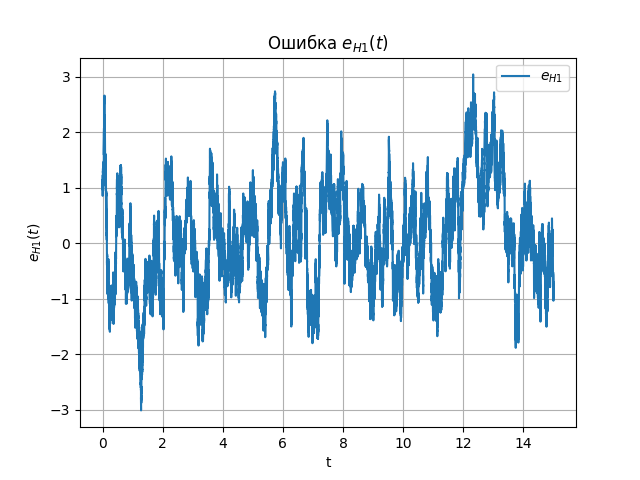
\includegraphics[width=0.8\textwidth]{images/eh1.png}
		\caption{График ошибки оценивания $e_{H1}(t)$}
		\label{fig:eh1}
	\end{figure}
	\begin{figure}
		\centering
		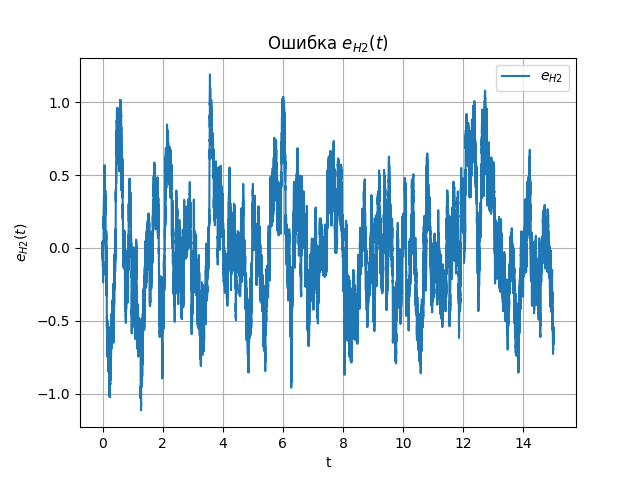
\includegraphics[width=0.8\textwidth]{images/eh2.png}
		\caption{График ошибки оценивания $e_{H2}(t)$}
		\label{fig:eh2}
	\end{figure}
	\begin{figure}
		\centering
		
\includegraphics[width=0.8\textwidth]{images/j.png}
		\caption{График значения квадратичного критерия $J(t)$}
		\label{fig:j}
	\end{figure}

	Можем видеть, что ошибки $e_{Hi}$ имеют случайный характер возле нулевого положения, а критерий качества даёт какие-то ненулевые значения - в целом картина ожидаемая.

	\section{Доказательство оптимальности}
	Теперь отклоним расчётные значения $L$ так, чтобы наблюдатель сохранил устойчивость. Возьмём следующие матрицы
	\[
		L' = L + \begin{bmatrix}
			1.25 \\ 1.25
		\end{bmatrix}, \quad L'' = L - \begin{bmatrix}
			1.25 \\ 1.25
		\end{bmatrix}
	\]

	Аналогично промоделируем их поведение при том же времени $t = 15$ секунд. Графики представлены на рисунках \ref{fig:eh1_suboptimal}-\ref{fig:j_suboptimal1}, а средние значения $J'(t)$ соответственно $J'\approx 1.5806$ и $J''\approx 1.7959$.
	\begin{figure}
		\centering
		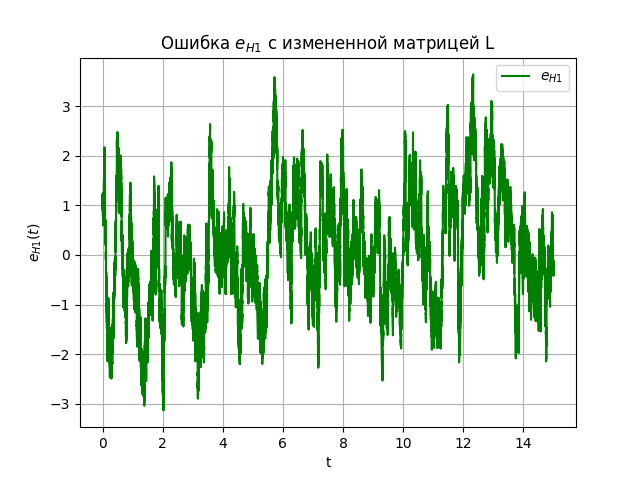
\includegraphics[width=0.8\textwidth]{images/eh1_suboptimal.png}
		\caption{График ошибки оценивания $e_{H1}(t)$ при $L'$}
		\label{fig:eh1_suboptimal}
	\end{figure}
	\begin{figure}
		\centering
		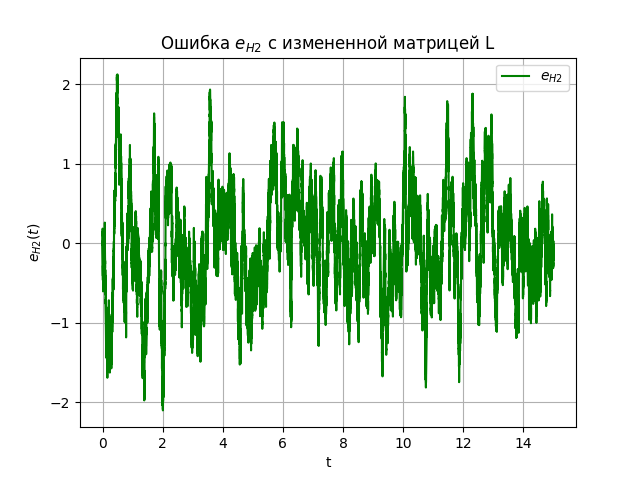
\includegraphics[width=0.8\textwidth]{images/eh2_suboptimal.png}
		\caption{График ошибки оценивания $e_{H2}(t)$ при $L'$}
		\label{fig:eh2_suboptimal}
	\end{figure}
	\begin{figure}
		\centering
		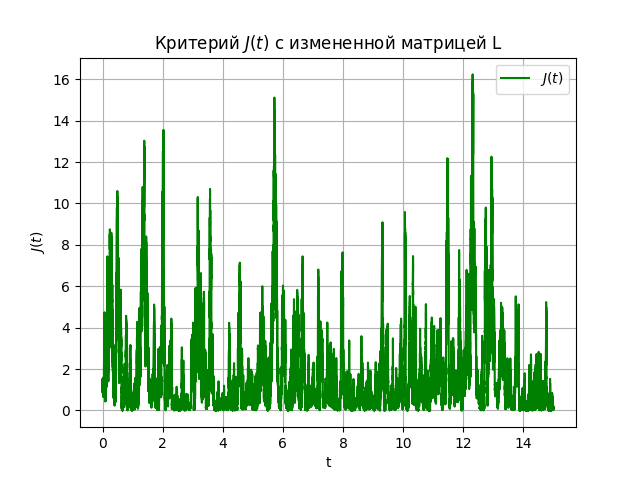
\includegraphics[width=0.8\textwidth]{images/j_suboptimal.png}
		\caption{График значения квадратичного критерия $J(t)$ при $L'$}
		\label{fig:j_suboptimal}
	\end{figure}
	
	\begin{figure}
		\centering
		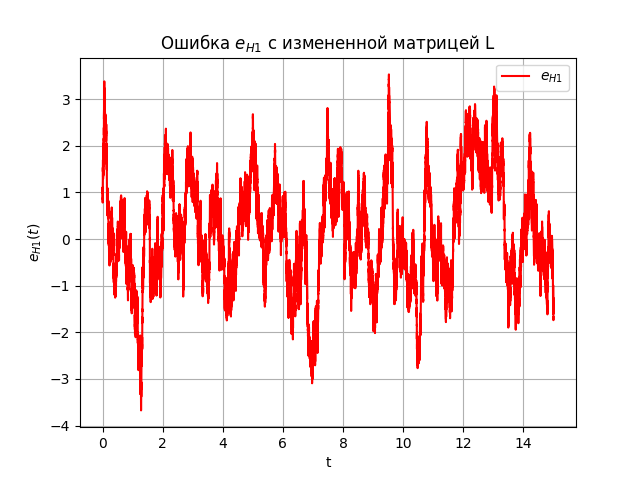
\includegraphics[width=0.8\textwidth]{images/eh1_suboptimal1.png}
		\caption{График ошибки оценивания $e_{H1}(t)$ при $L''$}
		\label{fig:eh1_sumoptimal1}
	\end{figure}
	\begin{figure}
		\centering
		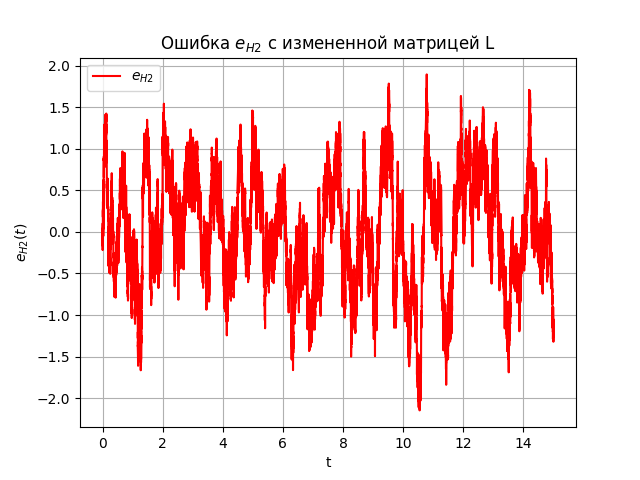
\includegraphics[width=0.8\textwidth]{images/eh2_suboptimal1.png}
		\caption{График ошибки оценивания $e_{H2}(t)$ при $L''$}
		\label{fig:eh2_suboptimal1}
	\end{figure}
	\begin{figure}
		\centering
		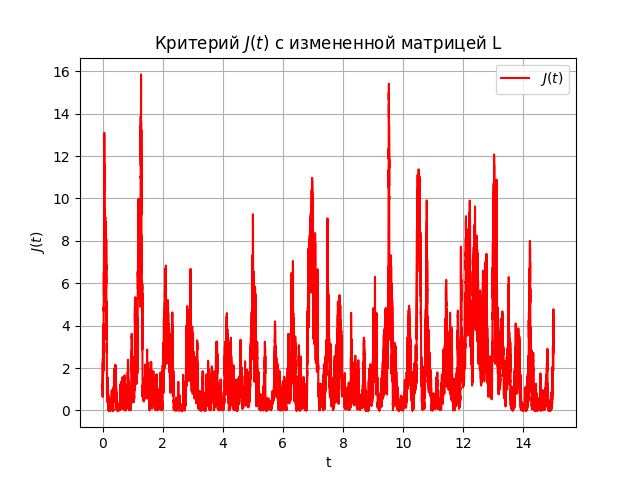
\includegraphics[width=0.8\textwidth]{images/j_suboptimal1.png}
		\caption{График значения квадратичного критерия $J(t)$ при $L''$}
		\label{fig:j_suboptimal1}
	\end{figure}

	Видим, что в среднем $J' > J$ и $J'' > J$ для $J$, найденного на предыдущем шаге, поэтому можем сказать, что в смысле критерия качества $J=M\{e_H^T e_H\}$ наблюдатель c матрицей усилений $L$ является оптимальным.

	Также стоит отметить, что чем более мы удаляемся от $L$, тем выше и это отклонение $J_{new} - J$, что ещё раз говорит об оптимальности построенного наблюдателя.
	
	\section{Изменение параметров шума}
	Теперь посмотрим, как матрицы $W$ и параметр $V$ влияют на наш наблюдатель. Для начала изменим $W$ до
	\[
		W' = 2 W = \begin{bmatrix}
			16 & 6 \\
			6 & 4
		\end{bmatrix}
	\]
	\begin{figure}
		\centering
		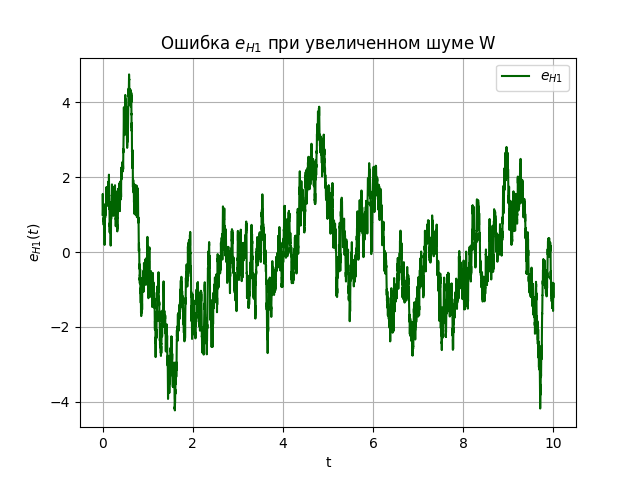
\includegraphics[width=0.8\textwidth]{images/eh1_w.png}
		\caption{График ошибки оценивания $e_{H1}(t)$ при $W'$}
		\label{fig:eh1_w}
	\end{figure}
	\begin{figure}
		\centering
		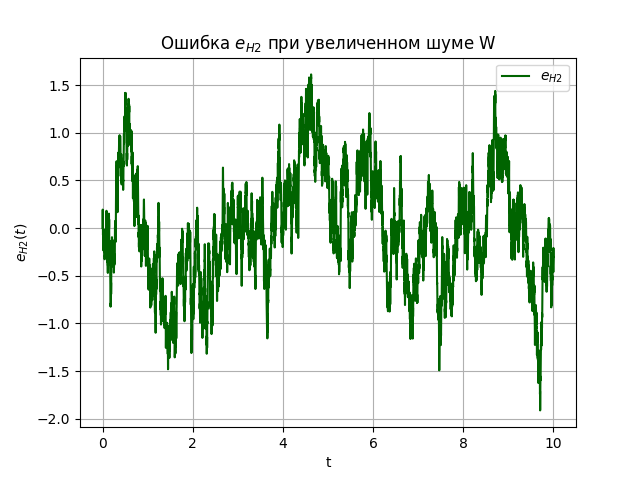
\includegraphics[width=0.8\textwidth]{images/eh2_w.png}
		\caption{График ошибки оценивания $e_{H2}(t)$ при $W'$}
		\label{fig:eh2_w}
	\end{figure}
	\begin{figure}
		\centering
		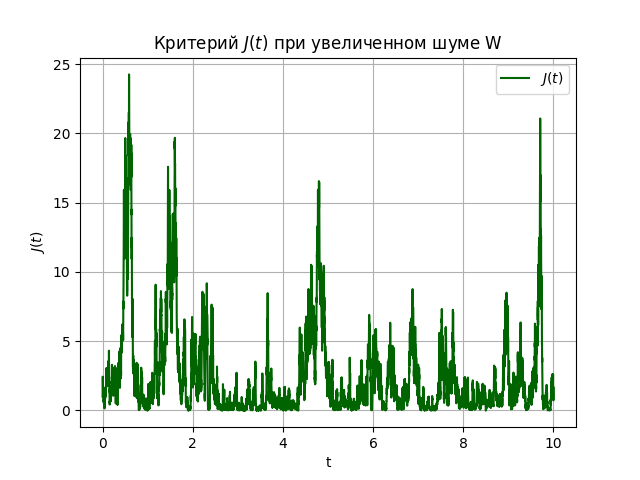
\includegraphics[width=0.8\textwidth]{images/j_w.png}
		\caption{График значения квадратичного критерия $J(t)$ при $W'$}
		\label{fig:j_w}
	\end{figure}
	Тем самым мы увеличим шум, приходимый на состояния $x_1$ и $x_2$ системы. Моделирование представлено на рисунках \ref{fig:eh1_w}-\ref{fig:j_w}. Отметим, что увеличился и критерий $J_{W'} \approx 1.8732$.

	Это означает, что наблюдатель стал работать значительно хуже. Увеличение шума, действующего непосредственно на состояния системы, напрямую и существенно снижает точность их оценки. Система становится более "непредсказуемой" для наблюдателя, что приводит к росту среднего ошибки оценивания $e_H$.

	Теперь отклоним и спектральную плотность $V$ до
	\[
		V' = 4 V = 12
	\]

	Тем самым мы увеличим шум, приходимый на выход $y$ системы. Моделирование представлено на рисунках \ref{fig:eh1_v}-\ref{fig:j_v}. Как и прежде, критерий качества немного увеличился до $J_{V'} \approx 1.0886$.
	\begin{figure}
		\centering
		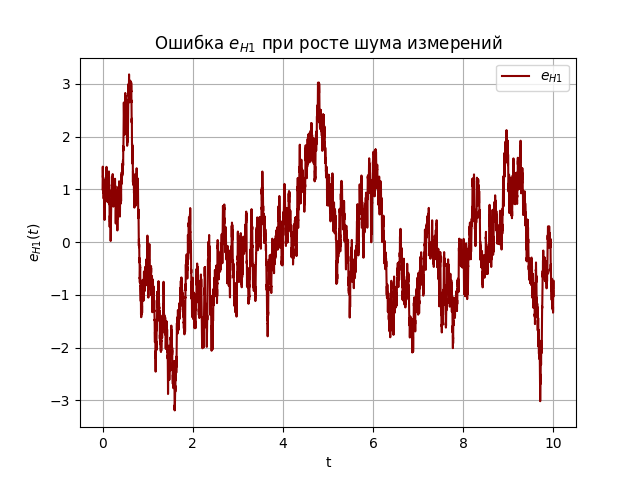
\includegraphics[width=0.8\textwidth]{images/eh1_v.png}
		\caption{График ошибки оценивания $e_{H1}(t)$ при $V'$}
		\label{fig:eh1_v}
	\end{figure}
	\begin{figure}
		\centering
		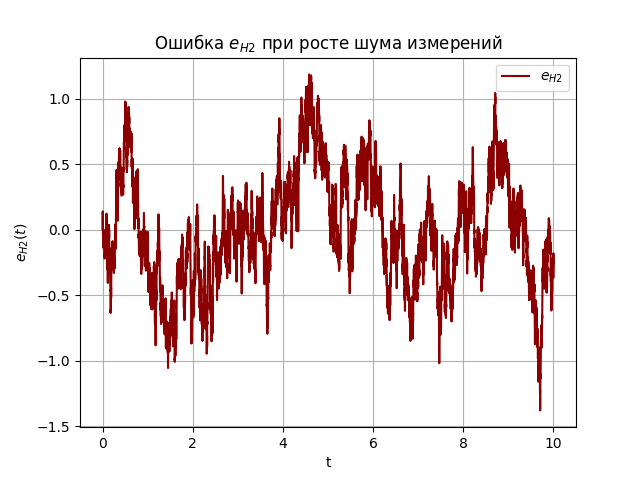
\includegraphics[width=0.8\textwidth]{images/eh2_v.png}
		\caption{График ошибки оценивания $e_{H2}(t)$ при $V'$}
		\label{fig:eh2_v}
	\end{figure}
	\begin{figure}
		\centering
		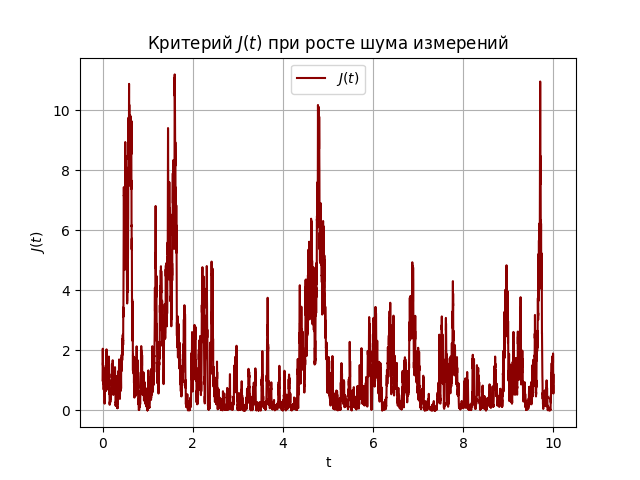
\includegraphics[width=0.8\textwidth]{images/j_v.png}
		\caption{График значения квадратичного критерия $J(t)$ при $V'$}
		\label{fig:j_v}
	\end{figure}

	Это показывает, что наблюдатель относительно устойчив к помехам в измеряемом сигнале. Несмотря на то, что выходной сигнал $y$ стал в четыре раза более "шумным", оптимальный наблюдатель все еще способен эффективно фильтровать этот шум и давать хорошую оценку состояния.

	\section{Проектирование LQG}
	Теперь мы можем объединить результаты построения оптимального наблюдателя с результатами построения оптимального регулятора (LQR), который вычислялся на основе уравнения Риккати относительно положительно определенной матрицы $P \succ 0$:
	\[
		\begin{cases}
			A^T P + PA + Q - P b r^{-1} b^T P = 0 \\
			K = r^{-1} b^T P	
		\end{cases}
	\]

	При принятых $Q \succcurlyeq 0$ и $r > 0$ из варианта
	\[
		Q = \begin{bmatrix}
			2 & 0 \\
			0 & 1
		\end{bmatrix}, \quad
		r = 5
	\]

	Откуда матрица обратных связей
	\[
		K = 
		\begin{bmatrix}
			1.8715 & 0.3934 
		\end{bmatrix}
	\]

	В итоге получим линейно квадратичный гауссовский регулятором $u=-K\hat{x}$ на основе наблюдателя состояния $\hat{x}$.

	Результаты моделирования приведены на рисунках \ref{fig:u_lqg}-\ref{fig:x2_lqg}. Для наглядности стабилизации были взяты начальные условия $x(0) = \begin{bmatrix}
		10 & -10
	\end{bmatrix}^T$. Можем видеть, что регулятор успешно справляется с поставленной задачей, стабилизируя систему лишь по выходу.
	\begin{figure}[h!]
		\centering
		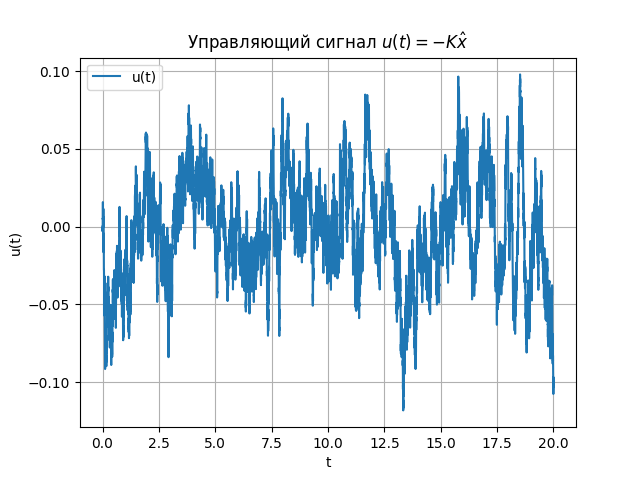
\includegraphics[width=0.8\textwidth]{images/u_lqg.png}
		\caption{График состояний $u(t)$ системы и наблюдателя}
		\label{fig:u_lqg}
	\end{figure}
	\begin{figure}
		\centering
		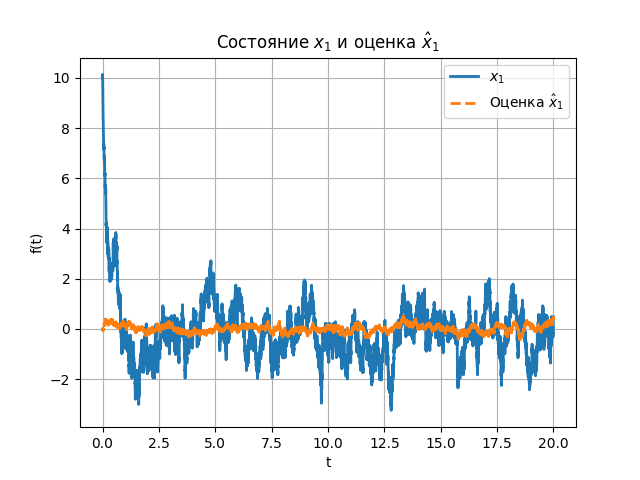
\includegraphics[width=0.8\textwidth]{images/x1_lqg.png}
		\caption{График состояний $x_1(t)$ системы и наблюдателя}
		\label{fig:x1_lqg}
	\end{figure}
	\begin{figure}
		\centering
		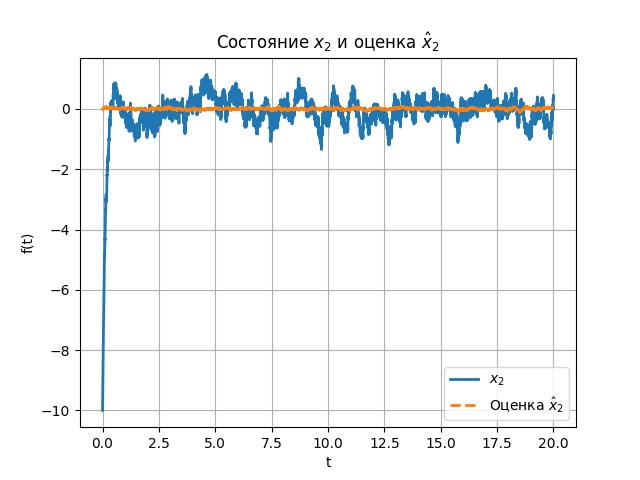
\includegraphics[width=0.8\textwidth]{images/x2_lqg.png}
		\caption{График состояний $x_2(t)$ системы и наблюдателя}
		\label{fig:x2_lqg}
	\end{figure}

	\section{Выводы}
	В ходе лабораторной работы был синтезирован и исследован оптимальный наблюдатель состояния для линейной системы, подверженной действию белых шумов. Его оптимальность была доказана путем сравнения квадратичного критерия ошибки с аналогичными показателями для наблюдателей с отклоненными параметрами. В заключение, на основе разработанного наблюдателя был успешно синтезирован и протестирован линейно-квадратичный гауссовский регулятор, который продемонстрировал эффективную стабилизацию объекта управления, используя только оценки состояния.
	



	
\end{document}